\chapter{Lecture 30 - Pressurizer Sizing Analysis}
\label{ch:ch30}
\section{Objectives}
The objectives of this lecture are:
\begin{enumerate}
\item Discuss the design basis for a typical PWR Pressurizer
\item Describe an analysis method for pressurizer sizing
\end{enumerate}

\section{Pressurizer Design Basis}
In a PWR, the pressurizer serves as an expansion volume for the primary coolant.  This is required since the water is essentially incompressible, and yet its density changes as a function of temperature.  Without the pressurizer, the primary coolant system would be subject to rapid and uncontrollable pressure fluctuations in response to small temperature variations.  A simplified schematic of the primary coolant system is provided for reference in Figure \ref{fig:primary-schematic}.
\begin{marginfigure}
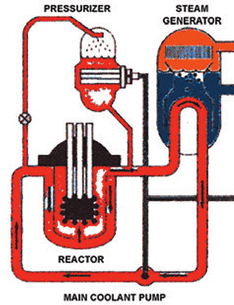
\includegraphics[width = 3.0cm]{primary-schematic.png}
\caption{Simplified schematic of primary coolant system.}
\label{fig:primary-schematic}
\end{marginfigure}

The pressurizer is maintained as a saturated system with a saturated steam bubble over a volume of saturated liquid water.  Electric heaters are installed in the lower portion of the pressurizer and used to maintain a steam bubble by evaporating primary coolant and generally increasing the temperature of the pressurizer. A spray system, which comprises relatively cool primary coolant piped in from the cold leg downstream of the reactor coolant pumps, is used to rapidly condense steam in the bubble to reduce system pressure. \marginnote{\textbf{Question for discussion:} How might you use the pressurizer system to perform a non-critical heat-up of the primary coolant system?}

\newthought{As a review} let us consider the change of water level in the pressurizer in response to routine power level changes:
\begin{itemize}
\item \textbf{Up-Power Maneuver:} In this case, the thermal energy extracted by the steam generator increases $\left(\dot{Q}_{S/G} \Uparrow \right)$ so that, temporarily $\dot{Q}_{S/G} > \dot{Q}_{\text{Rx}}$.  Since more energy is being extracted from primary coolant than is being added, $T_{\text{avg}} \Downarrow$.  For water, this means the average coolant density goes down, so the coolant volume contracts.  This results an \emph{outsurge} of water from the pressurizer, and $L_{\text{pzr}} \Downarrow$.  The pressurizer is a fixed volume, however, if water level goes down the steam volume must expand; this lowers pressurizer pressure $\left(P_{\text{pzr}} \Downarrow \right)$.  When this happens, saturated liquid in the pressurizer flashes to steam, mitigating the pressure drop.  If pressure falls low enough, the heaters are energized to create still more steam and further mitigate the pressure drop.

\item \textbf{Down-Power Maneuver:} For this case, the dynamics are the opposite.  $\dot{Q}_{S/G} < \dot{Q}_{\text{Rx}}$ so $T_{\text{avg}} \Uparrow$ resulting in an expansion of the primary coolant and $L_{\text{pzr}} \Uparrow$.  This \emph{insurge} compresses the steam bubble resulting an increase in $P_{\text{pzr}}$.  If pressure increases enough, spray flow will be engaged; relatively cool water partially condenses the vapor bubble thus reducing pressure.  When pressure falls below a specified set-point, spray flow is shut off.
\end{itemize}

For both up-power and down-power maneuvers, temperature feedback mechanisms result---in the short term, anyway---in re-equilibrium of $\dot{Q}_{\text{Rx}}$ and $\dot{Q}_{\text{S/G}}$ so that average coolant temperature and pressurizer water level ultimately return to their pre-transient level.  Any water that is added or removed from the primary coolant---for example, by coolant discharge to remove water or by coolant charging to add coolant---would result in the presserizer water level being increased or decreased respectively and this is undesirable.  Ideally, the pressurizer would be large enough to accomodate these transients without the need to add or discharge coolant and needlessly change pressurizer water level.

\newthought{This is basic} pressurizer dynamics.  Further consideration reveals the following points:

\begin{enumerate}
\item It is important that the pressurizer heaters not be uncovered.  If they are submerged in water, they can effectively transfer heat to water in the pressurizer and regulate pressure; if they are uncovered, their effectiveness is greatly reduced.

\item It is also important that the steam bubble never be fully collapsed.  For very rapid pressure transients, relief valves (some located in the pressurizer steam space) would open.  It is conceivable that a very rapid insurge could completely fill the pressurizer.  When this happens, spray flow would no longer be effective in reducing system pressure.
\end{enumerate}

\newthought{The overall goal} is to design the pressurizer so that, for ``foreseeable transients,'' the pressurizer is neither filled solid nor emptied to the point where the electric heaters would be uncovered.
The design question is: \emph{How big, then, should the pressurizer be?}

Clearly if the pressurizer is infinitely large, there will be no need to worry about filling solid or uncovering the heaters.  On the other hand, infinitely large pressurizers are expensive so some reasonable compromise must be made.

\section{AP1000 Pressurizer Design Basis}
As an example, let us consider the design basis for the AP1000 pressurizer.\sidenote{This is extracted from the AP1000 Design Control Document, Revision 19, Tier 2, Chapter 5, section 5.4.5.1 available at: https://www.nrc.gov/docs/ML1117/ML11171A454.pdf}

\begin{itemize}
\item The water volume is sufficient to prevent a reactor trip during a step-load increase of 10 percent of full power, with automatic reactor power. \marginnote{\textbf{Question:} What protective measure (influenced by the design of the pressurizer) would you expect to potentially cause a reactor trip due to the step-load increase?} 
\item The water volume is sufficient to prevent uncovering the heaters following a reactor trip and turbine trip, with normal operation of control systems and no failures of nuclear steam supply systems.
\item The steam volume is large enough to accommodate the surge resulting from a step load reduction from 100 percent power to house loads without reactor trip, assuming normal operation of control systems. \marginnote{\textbf{Question:} What protective measure (influenced by the design of the pressurizer) would you expect to potentially cause a reactor trip due to the step load decrease?}
\item The steam volume is large enough to prevent water relief through the safety valves following a complete loss of load with the high water level initiating a reactor trip, without steam dump.
\item A low pressurizer pressure engineered safety features actuation signal will not be activated because of a reactor trip and turbine trip, assuming normal operation of control and makeup systems and no failures of the nuclear steam supply systems.
\end{itemize}
As a result of these design bases, the AP1000 pressurizer is roughly 40 percent larger than pressurizers installed on previous PWRs of similar power level. \marginnote{\textbf{Question for discussion:} What are the operational pros and cons of having a big or small pressurizer?}

\section{Pressurizer Analysis Methodology}
We will employ the simplified control volume approach described in the Todreas text section 7.3.  The method calls for us to combine two separate analyses shown schematically in Figure \ref{fig:pzr-analysis-schematic}.
\begin{marginfigure}
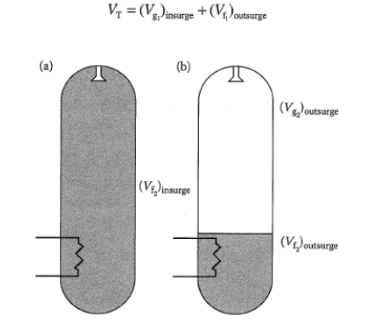
\includegraphics{pzr-analysis-schematic.png}
\caption{Schematic of insurge and outsurge final states for pressurizer size analysis.}
\label{fig:pzr-analysis-schematic}
\end{marginfigure}
\begin{enumerate}
\item \textbf{Insurge Analysis.}  We will size the pressurizer such that there is sufficient \emph{steam space} to accommodate a design-basis \emph{insurge} without filling the pressurizer solid.  This gives us a required volume of the steam space.
\item \textbf{Outsurge Analysis.} We will find the initial water volume such that a design-basis outsurge can occur without uncovering the heaters.  This gives us a required volume of the water-filled space.  
\end{enumerate}
The total pressurizer volume will be the sum of the steam volume and the water-filled volume obtained from those two separate analysis.  The outsurge analysis will also provide an estimate of the required pressurizer heater capacity.

\textbf{Disclaimer:} the analysis method to follow contains significant, and in some ways unrealistic, assumptions as well as access to system response parameters---such as \emph{mass of surged coolant} and \emph{mass of sprayed coolant}---that would require detailed system modeling to obtain.  Nonetheless, if one actually has access to such data, this method amounts to a way that you could use to obtain a preliminary estimate of pressurizer size. It is, perhaps, a little bit better than nothing.

\subsection{Insurge}
The design insurge will be modeled as a \emph{constant pressure} process. A temperature-entropy plot is shown in Figure \ref{fig:insurge-ts}; a schematic of the control volume is given in Figure \ref{fig:insurge-cv}.
\begin{marginfigure}
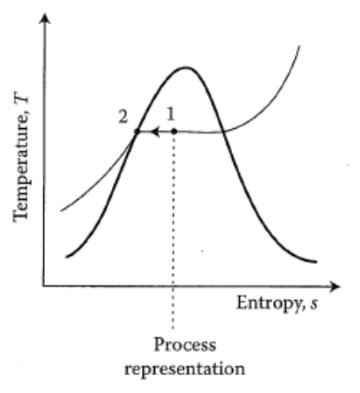
\includegraphics{insurge-ts.png}
\caption{Temperature-entropy plot for design basis insurge.}
\label{fig:insurge-ts}
\end{marginfigure}

\begin{marginfigure}
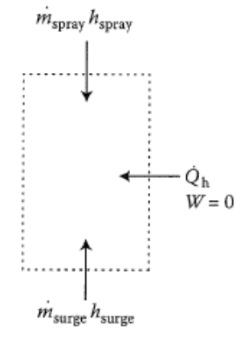
\includegraphics[width=2.25cm]{insurge-cv.png}
\caption{Control volume for design basis insurge.}
\label{fig:insurge-cv}
\end{marginfigure}

At the end of the transient, the entire pressurizer is filled with fluid, so the conservation of mass equation is given by:
\begin{equation}
m_{f_2} = m_{\text{surge}} + m_{\text{spray}} + m_{f_1} + m_{g_1}
\label{eq:insurge-com}
\end{equation}
where $m_{f_1}$ and $m_{f_2}$ is the mass of fluid at state point 1 and 2 respectively and $m_{g_1}$ is the mass of vapor at state point 1.  Let us define $m_{\text{spray}}$ as equal to $f m_{\text{surge}}$ where $f$ determined from system-wide modeling.  Then Equation \ref{eq:insurge-com} becomes:

\begin{equation}
m_{f_2} = m_{\text{surge}}(1+f) + m_{f_1} + m_{g_1}
\label{eq:insurge-com2}
\end{equation}

\newthought{The pressurizer} will remain at constant volume throughout the transient, so we can apply a volume constraint as given by Equation \ref{eq:insurge-vol}.

\begin{equation}
m_{f_2}\nu_f = m_{g_1} \nu_g + m_{f_1}\nu_f = (m_{\text{surge}}(1+f) + m_{f_1} + m_{g_1}) \nu_f
\label{eq:insurge-vol}
\end{equation}
where $\nu_f$ and $\nu_g$ are the specific volume of liquid and vapor respectively. The right-hand side makes use of the value of $m_{f_2}$ given by Equation \ref{eq:insurge-com2}.

We can combine the conservation of mass with the volume constraint to get an expression for $m_{g_1}$ which is:

\begin{equation}
m_{g_1} = \frac{m_{\text{surge}}(1+f)\nu_f}{\nu_g - \nu_f}
\label{eq:insurge-mg1}
\end{equation}

With a value for $m_{g_1}$, we can directly find the required vapor volume for the design-basis insurge by applying the specific volume of vapor:

\begin{equation}
V_{g_1} = m_{g_1}\nu_g
\label{eq:insurge-vg1}
\end{equation}

\newthought{Since energy} has to be conserved also, we need to calculate the required heater input to satisfy conservation of energy.  The basic conservation of energy equation for this system reads:


\begin{equation}
m_{f_2} u_f = m_{\text{surge}}(h_{\text{surge}} + fh_{\text{spray}}) + m_{g_1}u_g + m_{f_1}u_f + Q_h 
\label{eq:insurge-coe}
\end{equation}
where $Q_h$ is energy input from the heater.

Re-arranging Equation \ref{eq:insurge-coe} to solve for $m_{g_1}$, combining with Equation \ref{eq:insurge-mg1}, we can get an expression for $\dot{Q}_{h}$ as given in Equation \ref{eq:insurge-coe2}.

\begin{multline}
Q_h = \frac{m_{\text{surge}}(1+f)\left[\nu_g u_f - \nu_f u_g\right]  }{\nu_g - \nu_f} - \\ m_{\text{surge}} (h_{\text{surge}}+fh_{\text{spray}})
\label{eq:insurge-coe2}
\end{multline}

\marginnote{\textbf{Note:} We will find that this last result of $Q_{h}$ is not usually needed; it will provide the total heater power needed to ensure conservation of energy, but the corresponding result for the outsurge transient is expected to be much higher and set the real limit for what heater power capacity needs to be.  Nonetheless it is worthwhile---particularly considering the gross assumptions needed such as coming up with a value of $f$, for example---to ensure, at least, that $Q_h$ is a realistic non-negative number.}

\subsection{Outsurge}
The design basis insurge will also be modeled as a constant pressure process.  A temperature-entropy plot is shown in Figure \ref{fig:outsurge-ts}; a schematic of the control volume is given in Figure \ref{fig:outsurge-cv}.
\begin{marginfigure}
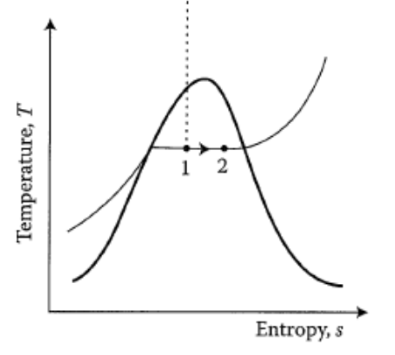
\includegraphics{outsurge-ts.png}
\caption{Temperature-entropy schematic for design-basis outsurge.}
\label{fig:outsurge-ts}
\end{marginfigure}

\begin{marginfigure}
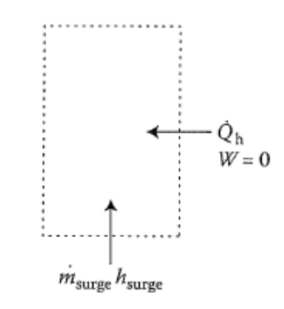
\includegraphics{outsurge-cv.png}
\caption{Control volume schematic for design-basis outsurge.}
\label{fig:outsurge-cv}
\end{marginfigure}

The conservation of mass equation for this outsurge is given as:

\begin{equation}
m_{f_2}+m_{g_2} = m_{f_1} + m_{g_1} - m_{\text{surge}}
\label{eq:outsurge-com}
\end{equation}
where, even though it is an outsurge, $m_{\text{surge}}$ is taken to be positive.

As with the insurge, we apply a constant volume constraint:

\begin{equation}
m_{f_2}\nu_f + m_{g_2}\nu_g = m_{f_1}\nu_f + m_{g_1}nu_g
\label{eq:outsurge-cov}
\end{equation}

Combining Equation \ref{eq:outsurge-com} and Equation \ref{eq:outsurge-cov} and we get:

\begin{equation}
m_{f_1} = m_{f_2} + m_{\text{surge}}\frac{\nu_g}{\nu_g - \nu_f}
\end{equation}
and, to get $V_{f_1}$:

\begin{equation}
V_{f_1} = m_{f_1}\nu_f
\label{eq:outsurge-vf1}
\end{equation}

Considering conservation of energy, we get:
\begin{equation}
m_{f_2}u_f + m_{g_2}u_g - m_{f_1}u_f - m_{g_1} u_g = -m_{\text{surge}}h_{\text{surge}} + Q_{h}
\label{eq:outsurge-coe}
\end{equation}
Through careful use of tedious algebra, we can solve for $Q_{h}$:

\begin{equation}
Q_{h} = m_{\text{surge}}h_{\text{surge}} - \left(u_f - \frac{\nu_f}{\nu_g}u_g \right)\left(m_{\text{surge}}\frac{\nu_g}{\nu_g - \nu_f} \right)
\label{eq:outsurge-q}
\end{equation}

\subsection{Summary}
This analysis provided a method for estimating required pressurizer size.  The initial vapor volume $V_{g_1}$ is obtained from Equation \ref{eq:insurge-vg1}; the required initial liquid volume $V_{f_1}$ is obtained from Equation \ref{eq:outsurge-vf1}; the total pressurizer volume is their sum.  The total energy input (during insurge or outsurge) is determined by the maximum value of $Q_h$ from design-basis insurge or outsurge transients.  For realistic system parameters, the $Q_h$ from outsurge should be larger.  Note, however, this is a heater energy input: we've said nothing about the time-scale for the insurge/outsurge transients so some additional analysis/estimates are needed to find required heater power.  As mentioned in the disclaimer, it is hoped that this analysis is somewhat better than nothing and provides some insight into how one might go about determining a reasonable estimate of required pressurizer size.



